\documentclass[../ei103948-project-documentation.tex]{subfiles}
\begin{document}
\section{Planificación del proyecto}
    \subsection{Spike o Iteración 0}

    A modo de anotación, también realizamos como iteración 0 un \textit{Spike} que utilizaba la tecnología del proyecto que hemos comentado anteriormente. A grosso modo un \textit{Spike} es un elemento del \textit{Product Backlog} orientado a la investigación o experimentación, cuya finalidad es obtener el aprendizaje necesario para implementar la funcionalidad solicitada por el cliente (en este caso los profesores de las asignaturas EI1039/48). A continuación se muestra un esquema jerarquizado donde se puede apreciar la estructura del \textit{Spike}. 

    \begin{figure}[H]
        \begin{center}
        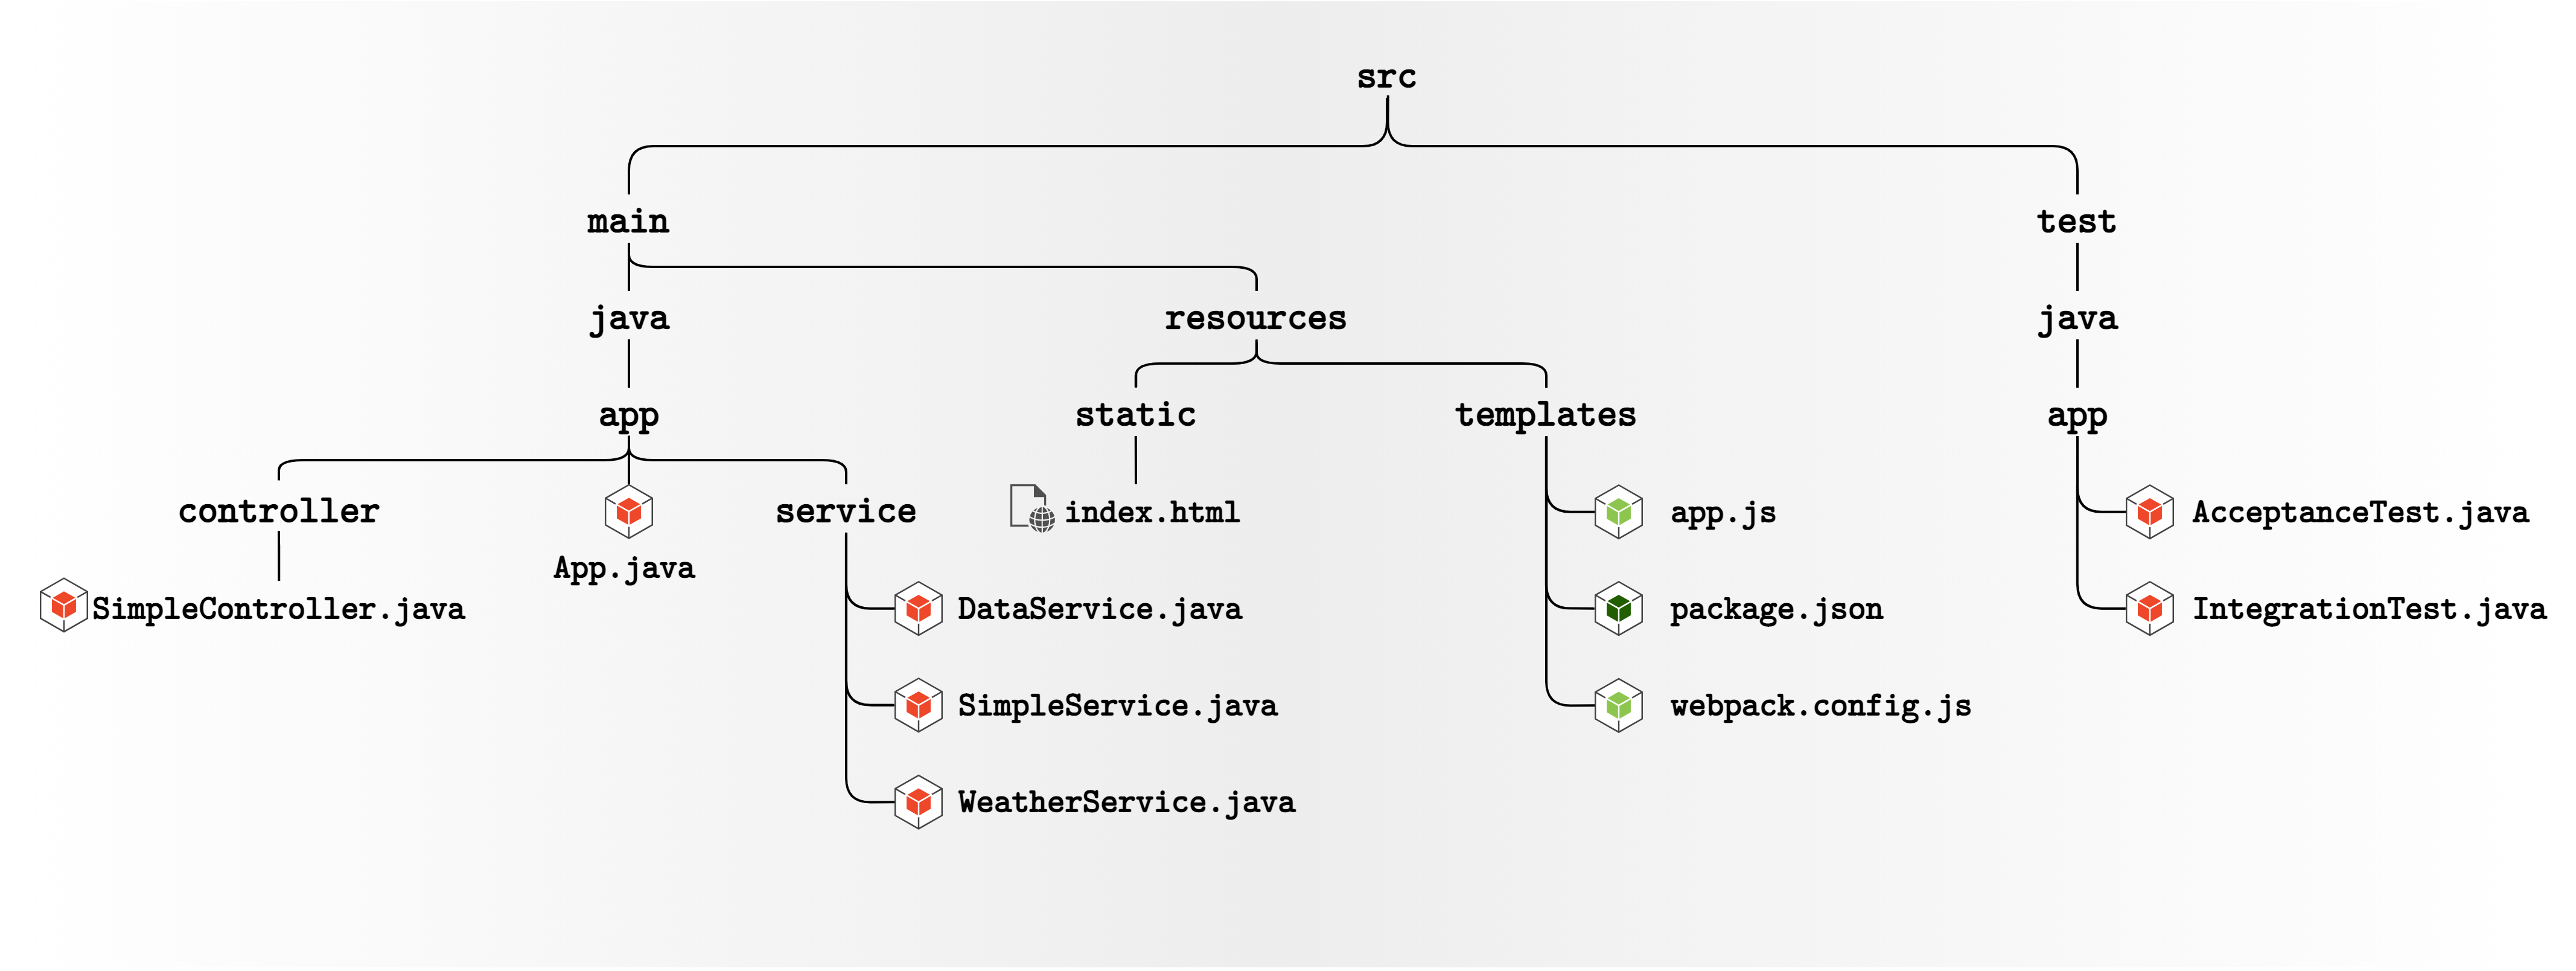
\includegraphics[scale=0.105]{images/jerarquiaSpike.png}
        \end{center}
        \caption{Jerarquía de archivos en el \texttt{Spike}}
    \end{figure}
    \subsection{Roadmap}

        A continuación y de forma esquemática, un pequeño \textit{roadmap} por las fases de iteración en el que los tests y servicios del proyecto van a ser implementados. El \textit{naming} de este apartado viene determinado por el siguiente patrón: \texttt{A.B.C.D}:
            \begin{itemize}
                \item \texttt{A}: Valores posibles: \emph{A-B}. Siendo un requisito Avanzado o básico.
                \item \texttt{B}: Número de requisito.
                \item \texttt{C}: Número de historia de usuario.
                \item \texttt{D}: (Si la hubiese): número de subhistoria de usuario.
            \end{itemize}

        \subsubsection{Iteración 1}
        La primera de las iteraciones hace referencia a los requisitos avanzados 1 y 2. Y es la que realizaremos antes de presentar la 2a entrega del proyecto. Las fechas de \underline{inicio} y \underline{final} son:
            \begin{itemize}
                \item [\faIcon{calendar-alt}] lunes, 8 de noviembre de 2021.
                \item [\faIcon{calendar-check}] viernes, 12 de noviembre de 2021.
            \end{itemize}
            \begin{enumerate}[\quad\quad\faIcon{check-circle}]
                \item A.R1.H1
                \item A.R1.H2
                \item A.R1.H3
                \item A.R1.H4
                \item A.R1.H5
                \item A.R2.H1
                
            \end{enumerate}

        \subsubsection{Iteración 2}
        La segunda de las iteraciones hace referencia a los requisitos básicos 1 y 3. Las fechas de \underline{inicio} y \underline{final} son:
            \begin{itemize}
                \item [\faIcon{calendar-alt}] lunes, 15 de noviembre de 2021.
                \item [\faIcon{calendar-check}] martes, 31 de noviembre de 2021.
            \end{itemize}
            \begin{enumerate}[\quad\quad\faIcon{check-circle}]
                \item B.R3.H1
                \item B.R3.H2
                \item B.R3.H3
                \item B.R3.H4
                \item B.R1.H3
                \item B.R1.H4
                \item B.R1.H1
                \item B.R1.H2
                \item B.R1.H10
                \item B.R1.H6
                \item B.R1.H7
                \item B.R1.H5
                \item B.R1.H9
                \item B.R1.H8
            \end{enumerate}

        \subsubsection{Iteración 3}
        La tercera y última de las iteraciones hace referencia al resto de requisitos básicos y avanzados. Esta iteración pone punto y final a la implementación de pruebas y servicios de esta aplicación; a margen de una semana de la entrega final, en esta iteración se pulirán todos los errores de cara a la clausura de este proyecto. Las fechas de \underline{inicio} y \underline{final} son:
            \begin{itemize}
                \item [\faIcon{calendar-alt}] miércoles, 1 de diciembre de 2021.
                \item [\faIcon{calendar-check}] miércoles, 15 de diciembre de 2021.
            \end{itemize}
            \begin{itemize}
                \item \textbf{Requisitos básicos}:
                \begin{enumerate}[\quad\quad\faIcon{check-circle}]
                    \item B.R2.H4.1
                    \item B.R2.H3
                    \item B.R2.H5
                    \item B.R2.H2.1
                    \item B.R2.H2.2
                    \item B.R2.H4.2
                    \item B.R2.H4.3
                    \item B.R2.H4.4
                    \item B.R2.H1.1
                    \item B.R2.H1.2
                    \item B.R4.H1
                    \item B.R4.H2
                    \item A.R3.H1
                \end{enumerate}
            \end{itemize}


\end{document}